\chapter{Introdução} \label{introducao}
\section{Contextualização}
Satélite é um termo utilizado para qualquer objeto que gira em torno de um corpo celeste em função da ação da força gravitacional. Ao longo dos anos, com o avanço da tecnologia, a humanidade desenvolveu e construiu centenas de milhares de satélites artificiais para cumprir diversos tipos de missões, por exemplo, aquisição de dados, monitoramento, posicionamento, telecomunicações, demonstrações, estudos meteorológicos, entre outros. Diariamente, milhões de pessoas consomem serviços que estão, direta ou indiretamente, relacionados com o funcionamento de algum satélite, não há dúvidas que os satélites artificiais permitiram que o mundo se tornasse uma grande aldeia.

Satélite artificial é qualquer dispositivo projetado para funcionar no espaço orbital da Terra, sendo que a principal variável a ser definida no desenvolvimento de um satélite é a sua missão, pois ela que guia boa parte das escolhas do projeto - órbita utilizada, formato, funcionalidades, tempo de vida, entre outras. Porém, para que esses dispositivos consigam prover alguma utilidade, todos têm uma infraestrutura em comum, o que inclui comunicação de dados, suprimento de energia, cálculo de posição, isso além das suas funções customizadas.\cite{nasa_comms_article} 

Este trabalho de conclusão de curso se enquadra dentro do projeto Alfacrux do laboratório LODESTAR da Universidade de Brasília (UnB). O projeto é uma iniciativa de pesquisadores e alunos que irá colocar em órbita baixa (aproximadamente 500 km de altitude) um nanossatélite até o final de 2023.

O projeto Alfacrux tem como um de seus objetivos desenvolver uma constelação de nanossatélites de comunicação em ondas curtas, ou seja, será possível trafegar sinais de voz e dados, porém em baixo volume, uma vez que o foco será prover comunicação em longo alcance para atingir áreas remotas. O nanossatélite será operado pela UnB atráves de bases em solo durante sua vida útil estimada de aproximadamente 2 anos, esse projeto é uma plataforma de interesse estratégico de parceiros como o Exercíto Brasileiro, uma vez que ele poderá ser utilizado, por exemplo, para fornecer comunicações em regiões remotas, a exemplo da Amazônia, onde não se tem infraestrutura ou interesse econômico em ofertar o serviço. 


\section{Objetivos}
\subsection*{Gerais}\label{gerais}

\noindent
\begin{minipage}{\linewidth}
\makebox[\linewidth]{
    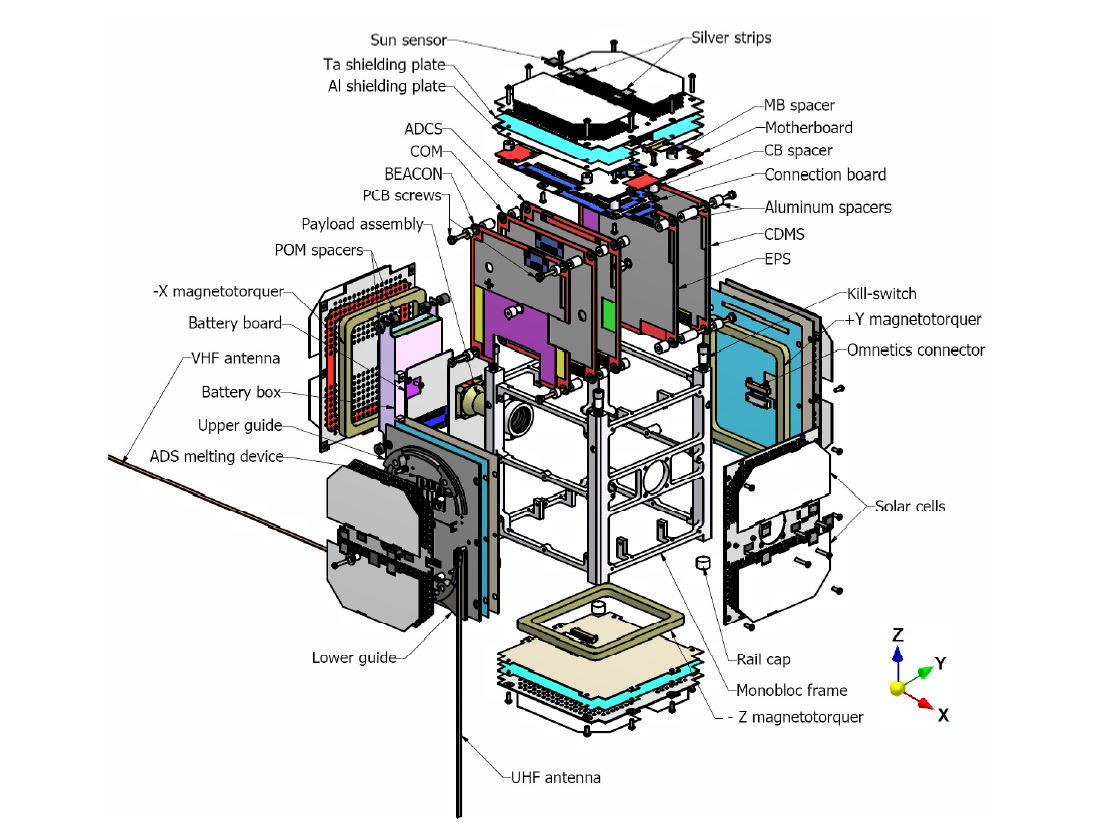
\includegraphics[keepaspectratio=true, scale=0.5]{imagens/Swisscube_exploded.png}}
\captionof{figure}{Visão explodida do nanossatélite Swisscube}
\label{swisscube_exploded_fig}
\end{minipage}

A imagem acima mostra a visão explodida do \textit{cubesat} Swisscube, que é uma das missões que utilizaremos como referência mais adiante, e nela podemos ver que um \textit{cubesat} é composto por vários módulos que desempenham funções distintas. Além de todos os módulos, existe o \textit{payload} do satélite, que é o componente relacionado com a missão que o satélite desempenha, por exemplo, se for uma missão de observação, o \textit{payload} será uma câmera, para uma missão de comunicação o \textit{payload} será um ou vários rádios e assim por diante. 

Existem módulos essenciais que normalmente aparecem em toda missão \textit{cubesat}, alguns exemplos são: OBC (On Board Computer) que é responsável por controlar as tarefas em curso no satélite, ADCS (Attitude Determination and Control System) responsável por determinar a atitude e mantê-la sob controle, podendo inclusive alterar a orientação para realizar melhores observações com câmera, melhor ganho de sinal para as transmissões de rádio, entre outras tarefas.

O Sistema Elétrico de Potência (EPS) é desses módulos essenciais para o funcionamento do \textit{CubeSat}, uma vez que ele é responsável por toda a gestão da energia do satélite, desde a aquisição, armazenamento e distribuição dessa energia. Normalmente, ele é dividido em duas partes principais, sendo uma responsável pelo carregamento da bateria atráves de panéis solares e uma segunda parte de que faz a regulação e distribuição das linhas de tensão necessárias para os demais módulos. 

O objetivo geral desse trabalho é propor uma primeira versão de um sistema EPS para os nanossatélites da constelação Alfacrux, respeitando as demandas enumeradas abaixo:

\begin{enumerate}
    \item Estar em concordância com o padrão \textit{CubeSat}.
    \item Possuir proteção contra subtensão e sobretensão da bateria.
    \item Possuir proteção contra sobrecorrente na linhas reguladas.
    \item Possuir sistema que maximiza a eficiência da placa solar.
    \item Possuir baterias para manter o satélite alimentado durante os períodos de eclipse.
    \item Possuir controle independente das linhas de alimentação.
    \item Possuir interface de comunicação com OBC - Computador de bordo.
    \item Permitir desenvolvimentos futuros.
\end{enumerate}{}


\subsection*{Específicos}\label{especificos}

\begin{enumerate}
    \item Levantamento dos requisitos de consumo.
    \item Levantamento das tarefas do nanossatélite.
    \item Dimensionamento da demanda de energia conhecendo o consumo esperado e as tarefas desempenhadas pelos módulos.
%    \item Levantamento das interfaces necessárias (entre a própria placa e também com outros sistemas do nanossatélite)
    \item Levantamento das condições de operação.
    \item Lista de especificações e componentes escolhidos para o projeto
    \item Simulações dos circuitos do EPS
%    \item Projeto da PCB
\end{enumerate}